%-------------------------------------------------------------------------
\section{Preliminary}
\label{sec:tracker-preliminary}

The problem of vehicle tracking in existing traffic surveillance video presents some unique computer vision challenges, including scale changes, video quality (exposure control, automatic white balance and compression), weather conditions, illumination changes, variations in perspective, and occlusion.
Current work in object detection 
\cite{viola2001rapid,dalal2005histograms,felzenszwalb2010cascade,girshick2014rich}, 
tracking \cite{henriques2015high,hare2011struck,vojir2014robust}
and background subtraction \cite{barnich2011vibe,zivkovic2006efficient}
% \cite{barnich2011vibe, zivkovic2004improved, zivkovic2006efficient, wang2007consensus} 
can deal with a subset of these conditions, but so far a generic system has been elusive. Below, we first introduce the underlying methods used in our system, then describe our vehicle tracking framework in detail. 

%We are inspired by the observation that object detector and background subtraction are complementary in some sense. Background subtraction model is able to catch small moving object but sensitive to illumination change and occlusion; on the contrary, object detector is robust to lighting and occlusion change, while prone to miss small object. Meanwhile, motion is a key evidence when appearance is not reliable and able to be computed efficiently as optical flow. We are trying to build a generalized form to combine these components into a reliable framework.

%-------------------------------------------------------------------------
\subsection{Background subtraction}
Background subtraction generates a binary foreground mask given a sequence of frames. Connected areas in the foreground mask can be treated as moving objects, although this technique can be error prone. 
We use ViBe \cite{barnich2011vibe}, for its balance of speed, robustness and accuracy. However, other methods 
% including \cite{stauffer1999adaptive, kaewtrakulpong2002improved,zivkovic2004improved,godbehere2012visual,kumar2000foreground, javed2002hierarchical,elgammal2000non,zivkovic2006efficient,wang2007consensus} 
could be substituted with acceptable results in many cases.

\ref{fig:tracker-bg} summarizes four common failure cases of the background subtraction with foreground bounding boxes on the original frame on the left and the foreground on the right. Automatic exposure (Figure \ref{subfig:bg-autoExposure}) is performed by the camera during recording, whereas illumination variation (Figure \ref{subfig:bg-illuminationChange}) is due to external light sources, such as the sun and vehicle headlights.
Both automatic exposure and illumination variation cause rapid and widespread changes in pixel values, which most background subtraction methods struggle with. 
Occlusion (Figure \ref{subfig:bg-occlusion}) creates a single connected foreground area out of two or more moving objects, or sometimes multiple foreground areas for a single moving object, breaking any assumption of a one-to-one mapping between foreground areas and moving object.
Ghosting (Figure \ref{subfig:bg-ghost}) usually happens when a foreground object remains stationary for a long time, during which time it is gradually assimilated into the background model.
When the object begins to move, what appears from behind the object is inaccurately marked as foreground, until the background model has had time to adjust.
% To make matters worse, it can take a long time for the model to correct this mistake, depending on the model's rate of adaptation, and the content of the video. 
%Once the background model fails, it is hard to extract the real moving object since it is just a pixel-level operation.
%, extra information like edge \cite{st2015subsense} and texture \cite{st2015self} may help to improve robustness. 
\begin{figure}[!htbp]
\centering
    \begin{minipage}{0.96\columnwidth}
        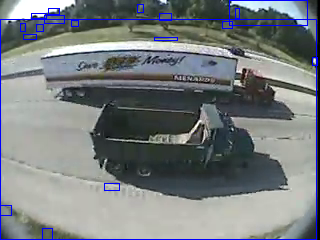
\includegraphics[width=0.48\linewidth, height = 0.3\linewidth]{./img/bg/252707.png}
        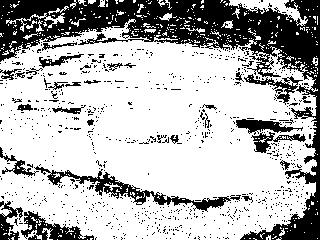
\includegraphics[width=0.48\linewidth, height = 0.3\linewidth]{./img/bg/252707_FG.png}
        \subcaption{Camera auto-exposure.}
        \label{subfig:bg-autoExposure}
    \end{minipage}
    \hspace{0.02\columnwidth}
    \begin{minipage}{0.96\columnwidth}
        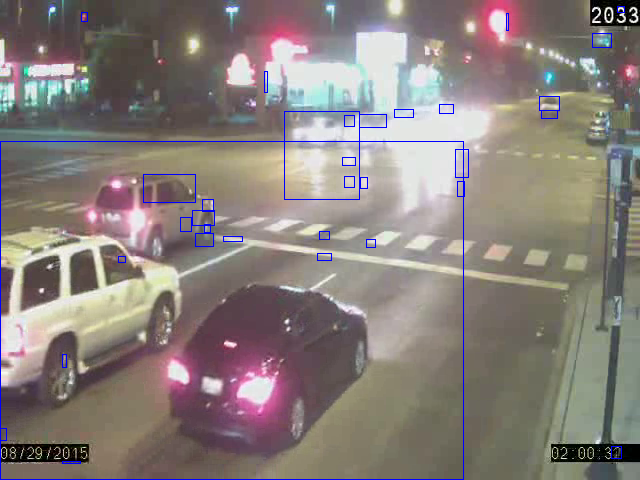
\includegraphics[width=0.48\linewidth, height = 0.3\linewidth]{./img/bg/ciceroPeterson.png}
        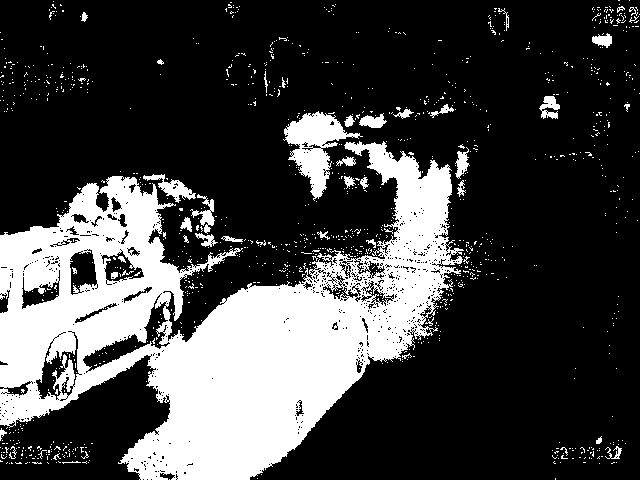
\includegraphics[width=0.48\linewidth, height = 0.3\linewidth]{./img/bg/ciceroPeterson_FG.png}
        \subcaption{Illumination change.}
        \label{subfig:bg-illuminationChange}
    \end{minipage}
    \vfill
    \begin{minipage}{0.96\columnwidth}
        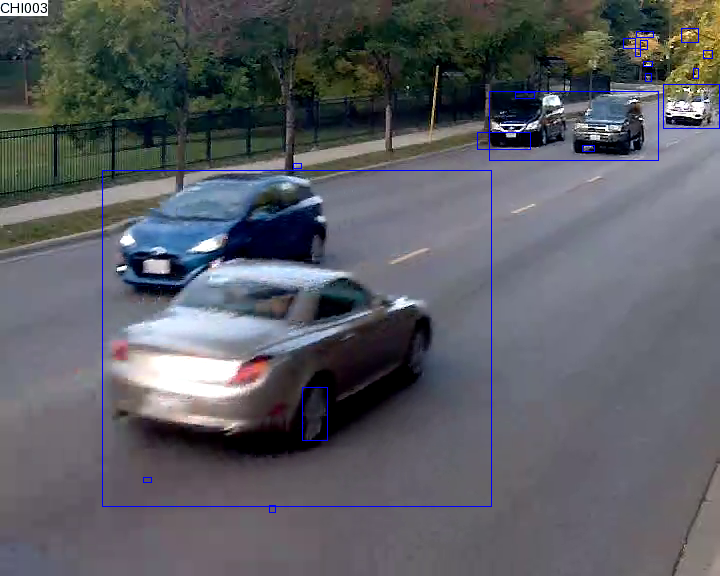
\includegraphics[width=0.48\linewidth, height = 0.3\linewidth]{./img/bg/ILCHI_CHI003.png}
        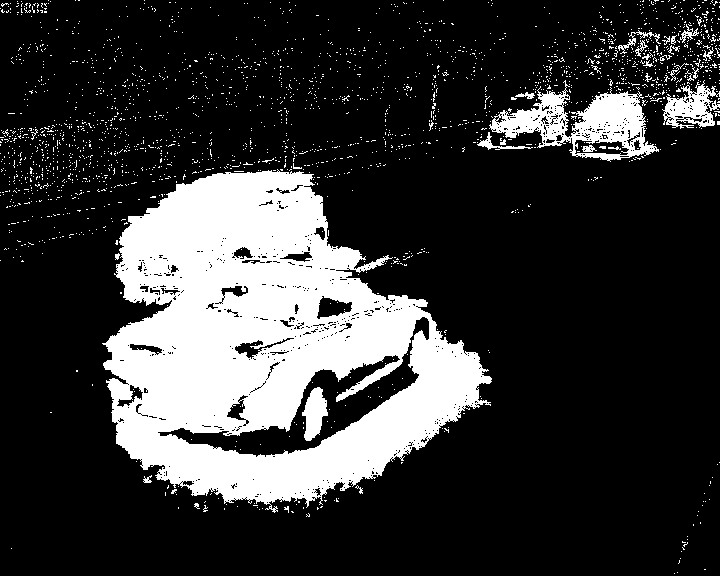
\includegraphics[width=0.48\linewidth, height = 0.3\linewidth]{./img/bg/ILCHI_CHI003_FG.png}  
        \subcaption{Occlusion. Note also the shadow, due to illumination change.} 
        \label{subfig:bg-occlusion}
    \end{minipage}
    \hspace{0.02\columnwidth}
    \begin{minipage}{0.96\columnwidth}
        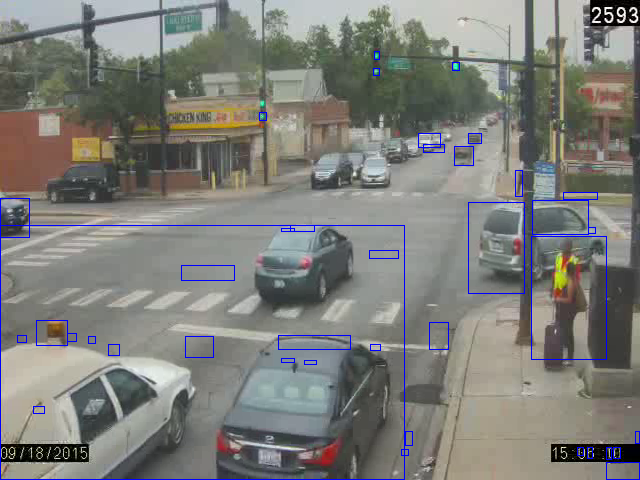
\includegraphics[width=0.48\linewidth, height = 0.3\linewidth]{./img/bg/halsted.png}
        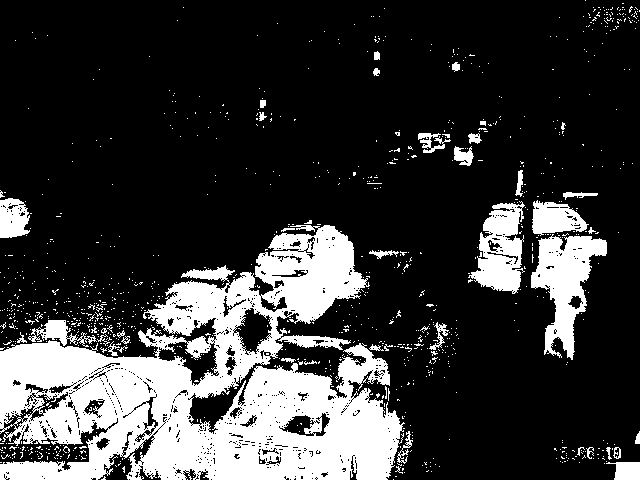
\includegraphics[width=0.48\linewidth, height = 0.3\linewidth]{./img/bg/halsted_FG.png}  
        \subcaption{Ghosting. Vehicles stopped at red light have become part of the background model.} 
        \label{subfig:bg-ghost}
    \end{minipage}
    %\vspace{-0.5em}
    \caption{Common background subtraction failure cases. Pixel values change for many reasons other than motion.}
    \label{fig:tracker-bg}
\end{figure}

In summary, background subtraction provides the ability to capture small movements without manual setup beforehand. However, it is error-prone and must be compensated by other methods to create a robust vehicle tracking system. 

%-------------------------------------------------------------------------
\subsection{Object detection}
\label{subsection:detector}

Object detectors \cite{felzenszwalb2010cascade,girshick2014rich} %viola2001rapid, dalal2005histograms
work on individual frames, scanning the image for areas that appear similar to offline training samples. 
Compared to background subtraction, object detection method tends to be more robust to illumination change and occlusion.
However, the cost of object detection is remarkable, as it often involves an exhaustive search throughout the image, both in location and object size.
%
%The detector usually works as a classifier after offline training, applied exhaustively on every possible window with different scales and ratios across the image. 
%The computation cost comes from the huge number of windows to check.
%Before the boosting of deep neural network, researchers were working on developing representative features.
Cascaded classifiers partially address this by discarding background regions \cite{felzenszwalb2010cascade}.
%Recently, with the development of GPU power and deep neural network architecture, both the feature and representation are greatly improved. 
%The state-of-the-art detector, called faster-RCNN \cite{renNIPS15fasterrcnn}, is used by our system. It integrates scan window filtering during forward passing. The time required for detection on one image drops from 2 seconds \cite{felzenszwalb2010cascade} to 198 ms on the PASCAL 2007 dataset, making real-time detection on videos possible.
More recently, deep neural networks \cite{girshick2014rich,renNIPS15fasterrcnn} have emerged as a promising approach to object detection. %he2014spatial, 
We use a state-of-the-art detector called faster-RCNN \cite{renNIPS15fasterrcnn}.
Running on a high-end graphics processing unit (GPU), the time required for detection on one image drops from 2 seconds \cite{felzenszwalb2010cascade} to 198 ms on the PASCAL 2007 dataset, making the real-time detection in video feasible. 
%It reduces detection time from 2 seconds \cite{felzenszwalb2010cascade} to 198 ms on the PASCAL 2007 dataset, making real-time detection on videos possible. 
However, like other detectors, faster-RCNN still has missing and false detections. In our measurements, it has a missing rate in excess of $65\%$ and $86\%$ on high- and low-resolution videos, respectively.
Thus, given the high miss rate, especially on poor quality images, object detection alone will not suffice for a robust vehicle tracking system. 

%\ref{fig:det_update} gives the number of total detection boxes and ground truth on videos with different resolutions. The detector misses a large number of objects, especially on low resolution videos. 
%This is because tiny vehicles in low resolution videos carry insufficient information for detector. 


% \textcolor{red}{not sure where to put this}such as Haar-like feature \cite{papageorgiou1998general} and HOG feature \cite{dalal2005histograms}.

%On the other hand, although more vehicles are detected on high resolution videos, only about $60\%$ detection boxes are used for tracking update. This indicates that the detector is not always stable and may have false detections.
% \begin{figure}[!htbp]
% \begin{center}
%   \includegraphics[width=\linewidth]{./img/track_detection_update_by_group.pdf}
% \end{center}
%    \caption{Detection count used during tracking.}
% \label{fig:det_update}
% \end{figure}
%-------------------------------------------------------------------------
\subsection{Optical flow}

Optical flow is an estimate of the movement of pixels between two images: in our case, two consecutive video frames. Optical flow provides a low-level description of motion in images and can offer useful evidence for tracking applications.
Estimating optical flow is a research area in its own right,
%\cite{zach2007duality, werlberger2009anisotropic, weinzaepfel2013deepflow}, but as many researchers before us, 
but we use the seminal Lucas-Kanade algorithm \cite{lucas1981iterative} in our system, as it runs fast on GPUs, and provides useful results while making minimal assumptions about the underlying scene and image. 
% in tasks like action detection or activity recognition. We use it to provide motion information besides appearance.
%The basic assumption of optical flow is brightness constancy constraints. 
% However, there is a common problem called \emph{aperture problem}, the local information is not sufficient to infer the global motion, since it is computed on a small neighborhood area. 
%To overcome this and achieve higher accuracy, smoothness constraints \cite{horn1981determining} and more complex regularization \cite{zach2007duality, werlberger2009anisotropic} is added. 
%According to \cite{weinzaepfel2013deepflow}, the current state-of-the-art optical flow algorithm requires $19\sim2000$ seconds for each pair of images. 
%For efficiency, we use the GPU version of Lucas-Kanade optical flow \cite{lucas1981iterative} in OpenCV \cite{opencv_library}.
\ref{fig:tracker-of} illustrates two optical flow problems that may affect tracking accuracy. The left column shows the direction and magnitude of the optical flow vectors, while the right column is the color code visualization of the optical flow results, with the color wheel at bottom right corner of Figure \ref{subfig:of-occlusion} indicating the corresponding direction. % in HSV color space. Direction corresponds to Hue value of the image, and magnitude corresponds to Value plane.
Figure \ref{subfig:of-aperture} illustrates the so-called aperture problem, where the center of the truck has no reported optical flow, due to its large and uniformly colored surface. %it is not likely to get an accurate movement estimation given such small area.
Figure \ref{subfig:of-occlusion} illustrates the ``turbulent'', error-prone flow that occurs where objects traveling in opposite directions meet.   %Since objects are represented as rectangles in our case, it is easy to include such erroneous flow once such case happens.

\begin{figure}[!htbp]
\centering
    \begin{minipage}{0.96\columnwidth}
        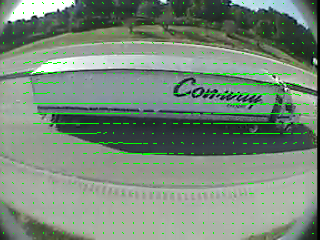
\includegraphics[width=0.48\linewidth, height=0.3\linewidth]{./img/of/252707.png} 
        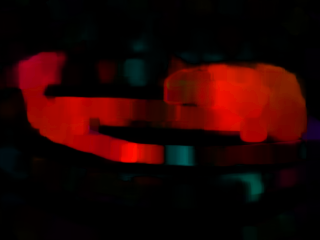
\includegraphics[width=0.48\linewidth, height=0.3\linewidth]{./img/of/252707_OF.png}
        \subcaption{Aperture problem.}
        \label{subfig:of-aperture}
    \end{minipage}
    \hspace{0.02\columnwidth}
    \begin{minipage}{0.96\columnwidth}
        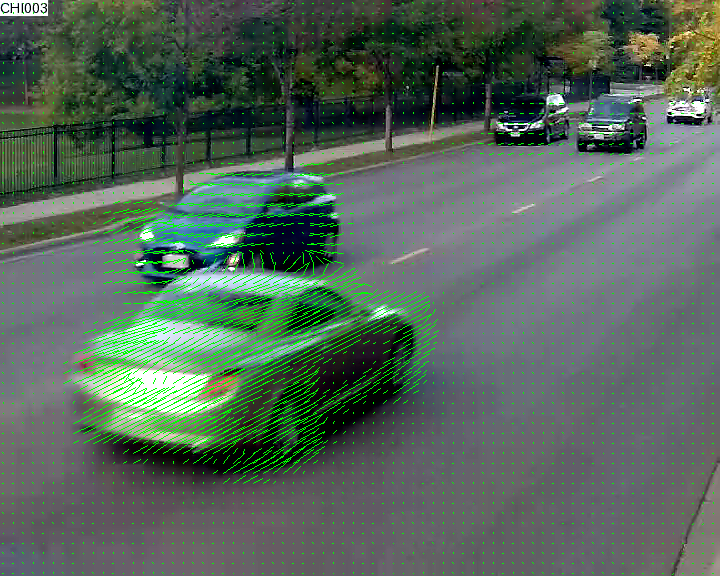
\includegraphics[width=0.48\linewidth, height=0.3\linewidth]{./img/of/ILCHI_CHI003.png}
        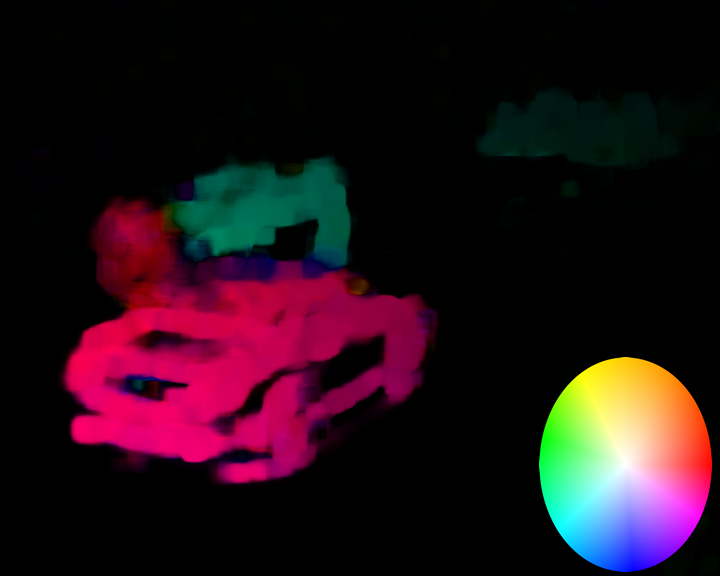
\includegraphics[width=0.48\linewidth, height=0.3\linewidth]{./img/of/ILCHI_CHI003_OF_wheel.png}
        \subcaption{Occlusion ``turbulence''.}
        \label{subfig:of-occlusion}
    \end{minipage}
    % \vspace{-0.5em}
    \caption{Common problems in optical flow estimation.}
    \label{fig:tracker-of}
    % \vspace{-0.5em}
\end{figure}

Thus, while {\it accurate} optical flow estimates offer valuable information about movement in the scene, it is neither complete (due to the aperture problem), nor free of severe estimation errors, in particular near occlusion boundaries. 
